% REMEMBER: You must not plagiarise anything in your report. Be extremely careful.

\documentclass{l4proj}

    
%
% put any additional packages here
%

\usepackage{pdfpages}

\begin{document}

%==============================================================================
%% METADATA
\title{A Distributed Game Using Adverts and Trackers In Web Browsers}
\author{Eftychios Karagiorgis}
\date{March 14, 2021}

\maketitle

%==============================================================================
%% ABSTRACT
\begin{abstract}
    Every abstract follows a similar pattern. Motivate; set aims; describe work; explain results.
    \vskip 0.5em
    ``XYZ is bad. This project investigated ABC to determine if it was better. 
    ABC used XXX and YYY to implement ZZZ. This is particularly interesting as XXX and YYY have
    never been used together. It was found that  
    ABC was 20\% better than XYZ, though it caused rabies in half of subjects.''
\end{abstract}

%==============================================================================

% EDUCATION REUSE CONSENT FORM
% If you consent to your project being shown to future students for educational purposes
% then insert your name and the date below to  sign the education use form that appears in the front of the document. 
% You must explicitly give consent if you wish to do so.
% If you sign, your project may be included in the Hall of Fame if it scores particularly highly.
%
% Please note that you are under no obligation to sign 
% this declaration, but doing so would help future students.
%
%\def\consentname {My Name} % your full name
%\def\consentdate {20 March 2018} % the date you agree
%
\educationalconsent


%==============================================================================
\tableofcontents

%==============================================================================
%% Notes on formatting
%==============================================================================
% The first page, abstract and table of contents are numbered using Roman numerals and are not
% included in the page count. 
%
% From now on pages are numbered
% using Arabic numerals. Therefore, immediately after the first call to \chapter we need the call
% \pagenumbering{arabic} and this should be called once only in the document. 
%
% Do not alter the bibliography style.
%
% The first Chapter should then be on page 1. You are allowed 40 pages for a 40 credit project and 30 pages for a 
% 20 credit report. This includes everything numbered in Arabic numerals (excluding front matter) up
% to but excluding the appendices and bibliography.
%
% You must not alter text size (it is currently 10pt) or alter margins or spacing.
%
%
%==================================================================================================================================
%
% IMPORTANT
% The chapter headings here are **suggestions**. You don't have to follow this model if
% it doesn't fit your project. Every project should have an introduction and conclusion,
% however. 
%
%==================================================================================================================================
\chapter{Introduction}

% reset page numbering. Don't remove this!
\pagenumbering{arabic} 

Ad Tracking and targeted advertising are part of the web browsing eco-system. While it is not essential to the personal browsing experience of a user, it is the main source of income for businesses that provide free services (such as Facebook). With this model, users can in most cases browse the web for free, but this comes at the cost of the user's privacy, and usually without their knowledge. 

Online targeted advertising is done on a massive scale, and many entities are involved in this processes, having access to a large number of internet users. As a result, mass amounts of user data is is being transported between these entities. Adding to this the fact that there is a general lack of transparency on what exact data is gathered from the user and how it is processed, serious privacy concerns are constantly being expressed (cite something that expresses privacy issues in targeted advertising).
TODO: Provide a bit more introduction to the project as well. Phrase the above paragrah a bit differently!

\section{Motivation}
The process of serving personalised adverts to the user starts from trackers that gather data about the user and share that data with advertisers. Advertisers then use that data to create an interest profile for users that is used to target personalised content in order to increase the likelihood that the user will be interested in their adverts with the hopes that the user will engage with that advert.

One of the privacy concerns with this process is that the user does not have much control over what data are used to create the interest profile or how the data are gathered, this leads into a very broad range of opinions and knowledge of targeted advertising systems.

In this paper, we attempt to use targeted advertising in a way that is fun and educational with the purpose of directly observing and improving the knowledge that users have of these systems. We also attempt to increase awareness of the various privacy and discrimination issues involved in these systems.
TODO: Refine motivation section, mention briefly privacy issues in targeted advertsing, maybe also mention any scandals that happened, and then tie it up with what we are trying to do in this paper.

\section{Aims}
In order to investigate and improve user knowledge of targeted advertising systems, we create a mutli-player game using adverts and third-party trackers in web browsers as game entities. The nature of the game is meant to be educational and experimental; We are not interested in building the most fun game, but rather explore the possibilities of using tracking and advertising in web browsers as game mechanics. During the game-play, players can put their knowledge to the test, with the goal of tricking the profiling done by advertisers or getting tracked by a certain amount of ad trackers, depending on the game mode. The two game modes that were implemented are as follows:

\textbf{Category mode:} Players are given an advert category that belongs to a content category (e.g Arts and Entertainment). Starting with a fresh browser account, they browse the web until they see an advert that belongs to the category given. This will allow the users to explore how the profiling is done by trying out different strategies to be targeted with an advert in that category. The first player to receive an advert in the given category is the winner. 

\textbf{Race mode:} Players browse the web with the goal of getting tracked by a certain number of distinct third-party ad trackers. Third-party trackers can be found in almost all types of websites, but some websites have a lot more trackers than others, which means the players can devise strategies that maximise the number of trackers identified, which effectively means that they have gained some insight as to which websites contain the most trackers. The first player to get tracked by the required number of distinct third-party ad trackers wins.

The nature of the game being multi-player allow players to discuss and collaborate with each other, which increases the engagement with the game and makes things more interesting. It also introduces a competitive factor to the game that can act as a motivator for users to improve their strategies.  Additionally, after the game, players can see what websites the other players have visited, which will be a good starting point for new players to come up with their own strategies.

In addition to the game-play, we include information sections in the game which are meant to help with improving the user's knowledge of tracking and targeted advertising systems by providing the necessary context that the user needs to understand what is happening while they are playing the game.     

In both game modes, we gather relevant gameplay metrics in order to analyse and evaluate the player's strategies. Additionally, using surveys, we evaluate the player's knowledge of targeted advertising systems before and after playing the game as well as the usability of the system in general. In particular, for the users that played the game, the key questions we would like to explore are:
\begin{itemize}
    \item
    What did the user know about targeted advertising systems and tracking, and what did they learn after playing the game?
    \item
    Did the user play the game blindly or did they have some sort of strategy in mind? What were the most visited types of websites by the users?
    \item
    If the user played multiple games, did their strategy improve over time?
\end{itemize}
TODO: The Aims section is better to be left for after the evaluation. 

\section{Content Structure}
We begin in Chapter 2 by providing an overview of related technologies and the state of affairs in online targeted advertising. In Chapter 3, we formalise the requirements and discuss the different aspects of the required solution. Chapter 4 shows the design decisions made along with explanations, it also gives an overview of the process throughout the production of the product and includes a high level overview of the system architecture. Chapter 5 dives into the implementation of the product, where the abstract details given in Chapter 4 are explained in more detail. We split the independent components of the system and explain their functionality and various challenges encountered throughout the development, we then give a complete picture of the system by putting everything together. In Chapter 6, we describe the experiment used the gathered data to help us make conclusions about the players knowledge of targeted advertising systems as well as the system's usability. Additionally, we analyse the gameplay for all the participants in any attempt to identify any patterns in their strategy. Finally, in Chapter 7 we discuss the limitations of our product and set the groundwork for future work. We end with a conclusion on the findings of this paper and a discussion as to why users need to have a better understanding of online targeted advertising systems.
TODO: Ensure this section is correct when paper is finished

%==================================================================================================================================
\chapter{Background}
In this chapter we provide a discussion on the entities involved in targeted advertising and how it works, as well as how trackers collect the user's data. While we are mostly interested in third-party trackers for the purpose of our game, we also explain how first-party tracking is usually done. Furthermore, we explain briefly the privacy risks and discrimination issues associated with targeted advertising and how they affects casual users. Finally, we explore technologies that are commonly used by users to deal with targeted advertising and we conclude with a section on related technologies to what we are trying to build.

\section{Targeted advertising systems}
\label{targeted}
In the early days of the internet, advertising was very limited due to the lack of user data and the lack of resources to display adverts on. This meant that advertisers would commonly place their adverts on any available media that existed, but rather than attracting users, it distracted them and annoyed them (\cite{earlyads}). With the modern advantages in recommender systems and the expansion of the internet with supporting technologies such as cookie matching or real-time bidding, advertisers can now use the context of the user to select what advert to serve to that user.    

\subsection{Entities involved in targeted advertising systems and their roles}
Targeted advertising systems are complex and there are a lot of entities involved that interact with each other in order to serve personalised adverts to users. \cite{Estrada-Jimenez2017}, discuss in detail how these entities interact with each other and what implications this might have in terms of privacy issues. Abstracting those details, let us first begin by giving a brief and simplified overview of how these systems work. 

Ultimately, the goal of these systems is to deliver the right ads to the right users. The entity responsible for promoting a service or product by serving ads to users are \textbf{advertisers}, but first they need a 'space' to display their advert so that they can maximise their reach of users. Typically, these spaces are provided by \textbf{publishers} and usually in the form of image banners in web pages with a redirection link to the website of the product or service being advertised. Publishers put these spaces on sale and they can either negotiate with advertisers to sell these spaces or have a real time auction to decide which advertiser is willing to give the best offer for a particular space at a particular point in time. It is through publishers that the users are exposed to the adverts. In practise, advertisers do not interact directly with the publishers but rather through ad platforms which provide interfaces that help advertisers and publishers improve their business plan and maximise their profit.

\textbf{Ad platforms} have evolved to make targeted advertising more efficient, transparent and flexible. This lead to more entities becoming involved to handle different parts of the systems. 

\textbf{Ad networks} are responsible for helping advertisers select the most optimal spaces for their adverts (an example of an ad network is GoogleAdSense).

\textbf{Ad exchanges} gather advert spaces from publishers and then using automated auctions, sell these spaces to the advertisers willing to pay the most. They also interact with the advertisers by sharing any data they have on the user that is currently being considered for a targeted advert, which is how the advertiser decides if they want to pay for a particular ad space or not. These auctions happen when the user is served content on a publisher's website and are extremely fast.

\textbf{Demand-side platforms (DSPs)} advise advertisers on what audience they should display their ads to and on what and platform. 

\textbf{Supply-side platforms (SSPs)} advise publishers on how to best use their spaces with the purpose of increasing profit and demand. 

Finally, \textbf{data aggregators} (trackers) are the entities responsible for collecting information about the users by tracking their online activity, which they share with ad exchanges. Ad exchanges then provide this information to the demand and supply-side platforms.

\subsection{Collecting data}
\textbf{First-party tracking} is done by publishers, usually for the purpose of collecting and analysing the user's information to offer a better experience with using their website. First-party tracking involves tracking the user using first-party cookies, which the user has to give consent before they could be used for advertising purposes. Cookies usually capture implicit data about the user's interactions with the website. Furthermore, data provided by the user, either directly through forms or captured from their network requests are also gathered.

\textbf{Third-party tracking} involves tracking the user by embedding content in first party websites (i.e in publisher sites) that allows trackers to monitor the user's browsing activity and capture meaningful data that will later on be used to target the user with personalised content. This content is usually embedded in the website without the user's consent, and in most cases, without the user's knowledge.
First-party tracking is less of a privacy concern than third-party tracking as it is limited to the users of the publisher's website. Additionally, there is usually more transparency as to what data is gathered and how it is used. The privacy risks in first-party tracking are directly correlated with the publisher's intentions; publishers can choose to sell private data to ad exchanges or use that data in malicious ways. Third-party tracking on the other hand is a much bigger privacy concern due to the lack of transparency and lack of user involvement. Finally, third-party trackers share the user's data with other entities in the targeted advertising eco-system, considering there is a vast amount of data moving between these entities, any potential data leaks can cause serious privacy issues. 

While different publishers and trackers collect different types of user information, and in some cases, there is no way to know for certain what exact data is gathered from the user, there are types of data that are commonly gathered when tracking the user (\cite{addata}):
\begin{itemize}
   \item 
   \textbf{Browsing Behaviour:}
   \begin{itemize}
	\item
           \textbf{Clickstream Data:} A record of web pages that the user has clicked on.
	\item
           \textbf{Search Data:} A record of search terms that the user has queried for.
	\item
           \textbf{Purchase Data:} A record of transactions that the user has either completed or started when using e-commerce sites such as Amazon.
	\item
           \textbf{Other:} Publishers may gather data about interactions of the user that are unique to their site. For example, Netflix gathers implicit data when the user's mouse hovers over an item (\cite{netflix}).
   \end{itemize}
   \item
   \textbf{Demographics:} Data such as the age, gender or education of the user.
   \item
   \textbf{Social Media Profile Data:} Any data the user has provided for their social media profiles such as their interests. 
\end{itemize}

\subsection{Process of serving personalised adverts to the user}
From the user's perspective, the ads that they see are part of the website they are visiting. The ads are indeed embedded in the content of the website, but the ads come from third party domains, and are served when the user's browser sends an HTTP request from the publisher's website. Since publishers are directly associated with ad exchanges, along with the original content that the user would have been served, additional content is served in the form of scripts or ad tags which are executed automatically by the browser. The scripts automatically notify the ad exchange, which in turn notifies advertisers that a space for adverts is available to be filled. Additionally, using cookie matching, ad exchanges can provide data about the user to the advertisers, and the ad space is then sold to the advertisers willing to pay the most, usually in real-time auctions in a process called real-time bidding (\cite{Estrada-Jimenez2017}).

This is a simplified view of how users get targeted with personalised adverts. In reality, many more of the entities mentioned in section \nameref{targeted} are involved in this process, with the ultimate goal of optimising the advertiser's and publisher's profit as well as maximising the perceived interest of the user for the advert to be served.

\subsection{Cookie Matching}
\textbf{Internet Cookies} are commonly used to store information about the user's visit to a website. There are two types of cookies: first-party cookies that are used by the publisher to remember important information about the user that would help improve their experience on that site, and third-party cookies that are used by domains other than the publisher's domain for tracking and advertising purposes (\cite{Estrada-Jimenez2017}). Since cookies contain information such as the user's search logs on a website, advertisers can use cookies to help them build the user's interest profile. 

\textbf{Cookie matching} is the process of identifying multiple cookies that belong to the same user and combining the information that those cookies contain in order to help advertisers select better adverts. To do this, ad exchanges place an identifier cookie on the user's pc when they first deliver adverts to the user. In subsequent visits of the user to websites associated with that ad exchange, the ad exchange extracts the identifier cookie and builds a mapping between that cookie and the user. Advertisers can then match their own cookies with the identifier cookie, effectively identifying the user and aggregating their information to form a better picture of the user's browsing activity. (\cite{Grandmont1985}).

\subsection{Real-time bidding (RTB)}
\textbf{Real-time bidding (RTB)} is an automatic process that happens when a user first visits a website that is associated with an ad exchange. The ad exchange notifies advertisers that a space is available for advertising and additionally, share the information they have about the user. The advertisers can then use the information shared by the ad exchange along with any information they already have about that user to decide if they want to bid on that ad space. This happens in a real-time auction (usually happens in fractions of a second) where multiple advertisers bid for the ad space and the advertiser who bids the most will have their advert displayed on that space (\cite{RTB}). Figure \ref{fig:rtb} shows the process of RTB and the different entities involved as well as the interaction between them.

\begin{figure}
    \centering
    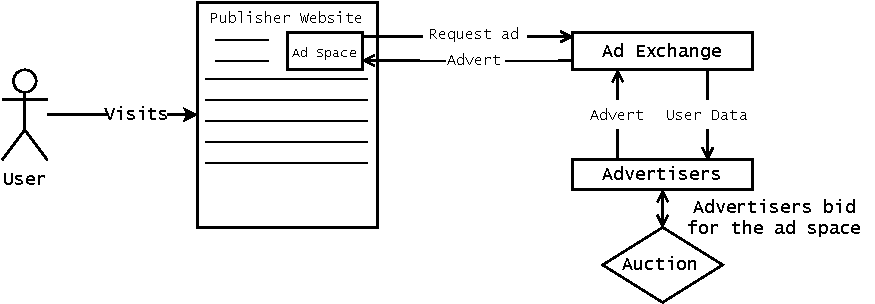
\includegraphics[width=1\linewidth]{images/RTB.pdf}    

    \caption{The process of RTB from the moment the user visits a Publisher website. }

    \label{fig:rtb} 
\end{figure}

\subsection{Privacy issues}
We have already discussed how the user's information is gathered in order to build the interest profile. This information can be stored and shared within the actors in the system, often with not enough precaution meaning that potential attacks or data leaks are possible, compromising the privacy of the user. The information can even be sold to third-party organisations, or used to manipulate politics. A good example of political manipulation in advertising is the Cambridge Analytica Data Scandal, where user data were gathered through an app and used to assist presidential political campaigns (\cite{cambridge}).

In a study to explore the sources of personally identifiable information that are used in targeted advertising, \cite{Venkatadri2019} identify a form of first party tracking where Facebook allows advertisers to target their users using personally identifiable information which users have uploaded to Facebook (such as their phone number) without being explicitly told that it can be used for advertising, showing the usual lack of transparency in targeted advertising. This paper also shows the lack of control on the user's site when it comes to selecting what exact data are they willing to share with advertisers. While in some cases, users might have the option to opt out of certain types of advertising, usually the user has no control at all.

Multiple complaints have been filled to regulators across the EU about RTB. One of the complaints, filed by Jim Killock and Michael Veal to the UK's Information Commissioner's Office (ICO) provided evidence that RTB can not comply with the Europe’s General Data Protection Regulation's (\cite{gdpr}) requirement to provide adequate security for the user's data and that RTB was in fact illegal. ICO shut down the complaint without taking any form of action or providing an adequate reason for not taking these complaints seriously (\cite{rtbcomplaint}). In fact, there has been a general lack of action by regulators to address the multiple complaints filed about RTB which is very problematic as it shows that the regulators are either not prepared to deal with these complaints or that they deliberately choose not to take any action for reasons that are not known (\cite{report}).

\subsection{Discrimination Issues}
\cite{Bol2019a} conducted an experiment with the purpose of identifying what advert categories groups of users with different demographics get targeted with. It was found that age, gender and education are all factors in targeted advertising, showing that these systems discriminate user groups in an attempt to maximise their efficiency. An implication of this form of discrimination is that it reinforces the usual age and gender stereotypes (e.g men like cars and women like beauty products). When presented with different discrimination scenarios, users stated that they found 44\% of them moderately or severely concerning and that discrimination based on demographics is more concerning than discrimination based on behaviour (\cite{Plane2017}).

This form of discrimination is very problematic as advertisers can take advantage of groups of people that are more suggestible to advertising due to their demographics. For example, constantly showing an older person adverts about skin care can be seen as a marketing strategy that aims to take advantage of the age of that person. While this is a form of personalised advertising, it can also be interpreted as a form of  high pressure advertising, where the advertisers exert persistent psychological pressure to force the user to interact with their advert (\cite{fennis2015psychology}).

% \section{Seams?}
% Can adverts be seen as seams in a browsing experience? Not in the traditional sense, as seams are more seen as aspects of a system that are often hidden from users to provide a more smooth experience. In this area of seams, there is usually some form of technical understanding that a user must have to interact more efficiently with the system

\section{Related products}
\subsection{Tally Saves The Internet Game}
Tally saves the internet is a browser game released in August 2020 that is implemented as a browser extension. When users have the extension installed and visit any website, it detects various tracking mechanisms and displays monsters somewhere on the page. The user has the option to fight the monster and defeat it in a turn-based RPG combat, which effectively blocks the trackers identified on the page. It also allows users to earn badges when finding different resources on the web or defeating different types of monsters.

Similar to Adblockers, the purpose of the game is to block tracking, advertising and the collection of the user's data in the browser. The biggest difference is that the game blocks trackers in an interactive manner, requiring the user's attention which ensures that the user is aware of the tracking done on that page (\cite{tally}). 

\subsection{Adblockers}
Users receive adverts as HTTP content through HTTP requests. The requests are made when a user accesses a publisher's site, and are out of the users control. This led to the development of browser add-ons that listen to these requests and block them, effectively blocking adverts from being served to the user. 

Ad blockers usually work by monitoring the user's HTTP traffic, and looking at the url of the domain that each request is made at. This url is then compared to a list that contains known advertiser domains and is either flagged as an advert or not, depending if the url is found in the list (an example of such a list is the EasyList). Alternatively, a domain can be flagged as an advert by identifying key words in the domain url. If the url is flagged as an advert, the ad blocker will block that request, which means the ad content will not be served to the user. Some ad blockers such as the AdBlockPlus chrome extension allow blocking additional traffic, where in addition to blocking requests made to known advert domains, they also block requests made to known tracker domains, which stops trackers from collecting the user's browsing activity.

Ad blockers are commonly used to block adverts that disrupt the user's browsing experience or block adverts with irrelevant or offensive messages. For example, when watching videos on YouTube, users are served with potentially non-skippable video adverts of varying length. In a study in the US in 2021 (\cite{stats}), it was found that 27\% of internet users were blocking adverts on their connected devices. 

Usually Ad blockers provide little or no control to the user in terms of filtering out a subset of adverts. For example, a user might have no problem being served adverts in any content category except gambling. In which case, they should have the option to only block adverts from advertisers that are serving gambling adverts. 

\subsection{AdReveal}
In an attempt to identify the different targeting mechanisms used in targeted advertising, \cite{Liu2013} performed an experiment to gather data about advert categories throughout various websites. To gather this data, user behaviour was simulated by using search logs gathered by AOL, which is an American online service provider. 
For each user in the search logs, the bing search engine was used to search for the items in the log and the top 5 websites were visited and advert information was collected using the AdReveal tool (a browser extension). The AdReveal tool scans the DOM of the website and gathers the following information: the url of the page and its semantic categories, the url the advert redirects to and its semantic categories and whether a re-marketing script is present on the page. The semantic categories of the pages are extracted by using a web categorisation API. 
This information was collected in two ways, in the first way, search history and cookies were wiped before the entirety of the search. In the second way, search history and cookies were wiped after each individual search. Using these data sets, a machine learning model was built and trained that predicts what kind of targeting mechanism was used for the adverts on the page by calculating a targeting score.

\subsection{Web Categorisation}
Web categorisation is the process of classifying a website into a finite set of predefined categories. This usually works by training a classification model in a supervised manner, which requires massive amounts of data for good performance. The data that the model trains on is HTML content of websites along with their categorisation. The model then learns the relationship between the keywords identified in the HTML content of a site and its categories. When training is finished, the model can then predict the categories of unseen websites using the knowledge it has gained (\cite{webcat}). It is worth noting that these models are not perfect, because the content of websites can vary a lot and there are websites that are extremely difficult to categorise, due to the ambiguity in their content. 

There are a lot of services that provide web categorisation APIs, which allow you to make HTTP requests to categorise a website using their pre-trained models by including the website's url in the request. The response will then either be no category, meaning that the model was not able to categorise the given website or a category (or a set of categories) that describes the content of the website.

\section{Summary}
In this section we have discussed how targeted advertising systems work and the entities and technologies involved in them. We have also discussed the various issues in these systems. These concepts are important for the development of the game, as they are the core of the game mechanics. 

The related products section looks at products that are either similar to what we have done or use methods that we have adapted for this project. The closest product to ours is Tally Saves The Internet Game but it is still very different to what we are trying to do. This project is unique in the sense that it is multi-player and uses both tracking and advertising as game mechanics. 

%==================================================================================================================================
\chapter{Analysis/Requirements}
What is the problem that you want to solve, and how did you arrive at it?
The problem is if we are somehow able to utilise adverts and trackers to create a fun, engaging and informative game (but with what purpose?). What is the information we already had on a high level? How did the research question/problem change over the course of the year. Any changes in the initial proposal (initial idea was to use Facebook but we went with web browser instead, why?).

\section{Initial Proposal and Refinements}
The requirements from the initial proposal involved playing the game in Facebook using fresh Facebook accounts rather than in the browser. Essentially, users would search for pages in Facebook with the purpose of tricking the profiling done by Facebook into categorising them in a way determined by the game itself. However, due to Facebook's guidelines and policies on new accounts and their authenticity, it was not feasible to use Facebook as the playing ground. This shifted the focus on using adverts in browsers instead.

Additionally, the idea of using trackers in the game in addition to adverts came later during the research phase of the project. It was apparent that tracking is a very important concept, and therefore, a new requirement was added to have a game mode involving tracking in browsers.

\section{User Stories}
For this project, we only have one set of user roles; the players. The user stories bellow reflect the requirements identified during the requirements analysis phase along with any requirements identified later on in the project. We split up the user stories into sections according to what the requirement is. These sections will be the different pages in the web app that the user would be able to navigate to.

\textbf{Authentication/Dashboard}
\begin{itemize}
    \item As a player, I want to be able to register and login, so that I can personalise the experience.
    \item As a player, I want to view game play metrics, so that I can see my progress.
    \item As a player, I want to view my game history, so that I can formulate a strategy based on my best performance.
    \item As a player, I want to be able to view all achievements, including those I have not yet completed, so that I know what achievements to aim for.
    \item As a player, I want to be able to change my password, so that I can ensure the security of my account.
    \item As a player, I want to be able to play the game anonymously, so that I can ensure my privacy.
    \item As a player, I want to be able to change my profile picture, so that I can choose which picture represents my account.
\end{itemize}

\textbf{Leaderboard}
\begin{itemize}
    \item As a player, I want to be able to view the leader board, so that I can see where I rank.
    \item As a player, I want to be able to search the leader board, to see the rank of a specific player.
\end{itemize}

\textbf{Lobby}
\begin{itemize}
    \item As a player, I want to join a lobby before the game, so that I can prepare for the game.
    \item As a player, I want to be able to chat with others before the game, so that I can socialise.
    \item As a player, I want to be able to indicate when I am ready, so that the game does not start without me.
    \item As a player, I want to be able to leave the lobby, in case something comes up.
    \item As a player, I want to be able to vote on the winning condition, so that I can have some control over the gameplay.
    \item As a player, I want to view the winning condition, so that I can formulate a strategy.
    \item As a player, I want to be able to see a helpful status message in the lobby, so that I know when I can start the game.
\end{itemize}

\textbf{Gameplay}
\begin{itemize}
    \item As a player, I want to view the status of the game at all times, so that I can know when the game ends.
    \item As a player, I want to be able to see other player's score, so that I am aware of the state of the game.
    \item As a player, I want to be able to chat with others while playing, so that I can discuss strategies.
    \item As a player, I want to be able to leave the game, in case something comes up.
    \item As a player, I want to be able to play different game modes, so that I can vary my game play.
    \item As a player, I want to be able to earn achievements while playing, so that I am motivated to play.
\end{itemize}

\textbf{Summary}
\begin{itemize}
    \item As a player, I want to be able to view a summary after the game, so that I know who won.
    \item As a player, I want to see the pages I and the other players have visited, so that I can come up with better strategies in future games.
    \item As a player, I want to be able to chat in the summary, so that I can discuss the game with other players.
\end{itemize}

\textbf{Other}
\begin{itemize}
    \item As a player, I want to be able to find information about the game, so that I know how to play.
\end{itemize}

\section{Functional Requirements}
We will now refine the user stories into implementable tasks which we categorise using the MoSCoW prioritisation technique (\cite{moscow}) that labels the tasks into Must Have, Should Have, Could Have and Won't Have according to their relative importance for the functionality of the system. We number the requirements so that we can reference them throughout the paper.

\textbf{Authentication/Dashboard}
\begin{enumerate}
    \item \textbf{Must Have:} Users must be able to register an account and log in the system.
    \item \textbf{Must Have:} Users must be able to view game metrics in the dashboard.
    \item \textbf{Should Have:} Users should be able to view their game history.
    \item \textbf{Should Have:} Users should be able to view all achievements available for them to complete as well as those they have already completed.
    \item \textbf{Must Have:} Users must be able to change their password.
    \item \textbf{Must Have:} Users should be able to create an account without providing personally identifiable information.
    \item \textbf{Could Have:} Users could be able to update their profile pictures.

\textbf{Leaderboard}
    \item \textbf{Should Have:} Users should be able to view the leader board.
    \item \textbf{Should Have:} Users should be able to search the leader board.


\textbf{Lobby}
    \item \textbf{Must Have:} Users must be able to join a lobby before the game.
    \item \textbf{Must Have:} Users must be able to chat with other players during the lobby.
    \item \textbf{Should Have:} Users should be able to indicate that they are ready before the game can start.
    \item \textbf{Must Have:} Users must be able to leave the lobby.
    \item \textbf{Could Have:} Users could be able to vote on the winning condition in the lobby.
    \item \textbf{Must Have:} Users must be able to see the winning condition in the lobby.
    \item \textbf{Must Have:} As a player, I want to be able to see a helpful status message in the lobby, so that I know when I can start the game.


\textbf{Gameplay}
    \item \textbf{Must Have:} Users must be able to see the status of the game while playing.
    \item \textbf{Must Have:} Users must be able to see the score of other players while playing.
    \item \textbf{Must Have:} Users must be able to chat while playing.
    \item \textbf{Must Have:} Users must be able to leave the game.
    \item \textbf{Should Have:} Users should be able to play multiple game modes.
    \item \textbf{Should Have:} Users should be able to complete achievements.

\textbf{Summary}
    \item \textbf{Must Have:}  Users must be able to view a summary of the game when the game ends.
    \item \textbf{Should Have:} Users should be able to see the pages they and the other players have visited.
    \item \textbf{Must Have:}  Users must be able to chat with other players in the summary page.
\textbf{Other}
    \item \textbf{Must Have:} Users must have the ability to read information about the game before playing.

\end{enumerate}

\section{Non-Functional Requirements}
In addition to the implementable tasks identified, we also identify tasks that are related to the behaviour of our system rather than what the user should be able to do. These requirements are few, but are very important for the functionality of the system.  

\begin{enumerate}
    \item \textbf{Must Have:}  The system must be able to handle updates to the game state in real time.
    \item \textbf{Should Have:} The system should be easy to use for new users, without requiring a lot of background information.
    \item \textbf{Must Have:} The system must be able to handle multiple games at the same time.
    \item \textbf{Must Have:} The system must only store information that is not sensitive and only relevant to the gameplay.
\end{enumerate}

\section{User Journey}
To give a more practical overview of the requirements, we provide a brief overview of the user's journey from account creation to playing the game. We include the requirements that have to be implemented under each step.
User journey:
\begin{enumerate}
    \item The user registers for an account and logs in
    \begin{itemize}
 	\item \textbf{Requirements: } [\#1, \#5, \#6 ]
    \end{itemize}
    \item The user reaches the dashboard
    \begin{itemize}
 	\item The dashboard shows the user's achievements, their game history and game-play metrics (such as games played, total number of trackers found, etc...)
           \item The leaderboard is also accessible from the dashboard
	\item It also has relevant information on how to play the game and a 'Find Game' button 
 	\item \textbf{Requirements: } [\#2, \#3, \#4, \#7, \#8 ]
    \end{itemize}
    \item The user reads how to play and searches for a game
    \begin{itemize}
 	\item \textbf{Requirements: } [\#25 ]
    \end{itemize}
    \item When a game is found, the user is put inside a lobby
    \begin{itemize}
 	\item The lobby allows users to chat with each other before the game starts
           \item It also informs the users what the winning condition is (i.e number of unique trackers to get tracked by or advert category depending on game mode)
           \item Users must indicate that they are ready before the game can start
 	\item \textbf{Requirements: } [\#9-15 ]
    \end{itemize}
    \item When all users are ready, they can start the game
    \begin{itemize}
 	\item During the game, the users visit websites and can see the current state of the game 
           \item The users can also chat during the game through the lobby
 	\item \textbf{Requirements: } [\#16-21 ]
    \end{itemize}
    \item A winner is found and the users get redirected to a summary page
    \begin{itemize}
 	\item The summary page uses the final game state to build relevant gameplay metrics that the users can see  
           \item User achievements, metrics and game history are updated
           \item Users have the option to leave the summary or play again
 	\item \textbf{Requirements: } [\#22-24 ]
    \end{itemize}
    \item Users leave the summary and are redirected to the dashboard
    \begin{itemize}
        \item In the dashboard, they can view their updated achievements, metrics and game history
    \end{itemize}

\end{enumerate}


%==================================================================================================================================
\chapter{Design}
In this chapter we provide an overview of the system and how the various components of the system interact with each other. Then, for each of these components we discuss the design details for the most notable parts. Finally, we discuss important aspects that are common to all the components. 

\section{Overview}
A high level explanation of the full system with the three different components (server, client and extension) and a simple, comprehensive diagram showing the interaction between these components.
\subsection{System Components}
When designing the infrastructure of the system, the requirements that limited the scope of technologies to use were the fact that the game must be multi-player and played in web browsers. The only way to fulfil these requirements is to implement the game as a web application. There was an apparent issue however; to build the gameplay logic, we need a way to monitor the user's browsing activity in sites outside of our domain which can not be done with front-end or back-end technologies. This led to the addition of another component into the infrastructure of the system; the browser extension, which gives us access to the user's network requests which we use to identify third-party trackers, and the HTML of each site the user visits during the game which we use to identify adverts.

The system can then be logically split into three high level components; the server, the client and the browser extension. These components work together to form the complete system where users can create accounts and play the game.
\begin{itemize}
    \item
    \textbf{Client:} This will be the front-end that will allow users to interact with the system.
    \item
    \textbf{Server:} The server will handle all network requests, along with any database operations. Additionally, the server will handle the communication between the clients and the extensions to handle updates to the game states for each player.
    \item
    \textbf{Browser Extension:} The extension will handle all gameplay logic and provide feedback to the players of the current game state.
\end{itemize}

\subsection{System Architecture}
Explain the interaction of the components of the system and include a system architecture diagram.
Figure \ref{fig:sysarch} shows the system architecture diagram with the three components and the interactions between them. The three components of the system interact in two different ways:
\begin{itemize}
   \item
   \textbf{HTTP requests:} Both the client and the extension interact with the server through HTTP requests. The client interacts with the server to authenticate users, retrieve database data and handle any functionality of the web application outside the game. The extension interacts with the server to retrieve the user's information as well as for categorising adverts identified during the gameplay.
   \item
   \textbf{Websockets:} To handle three-way, real-time communication between the components of the system, we use Websockets. Websockets allow us to set up TCP communication lines between the clients and the server and communication lines between the extensions and the server. Note that there is no direct communication line between the extensions and the clients, the server acts as an intermediary when these component want to communicate. 

\begin{figure}
    \centering
    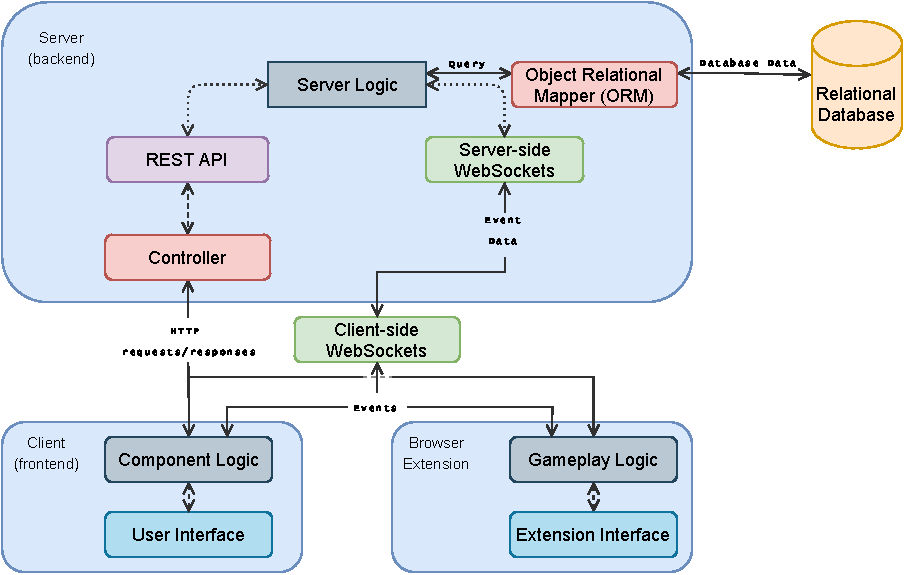
\includegraphics[width=1\linewidth]{images/sys_arch.pdf}    

    \caption{System Architecture diagram with the three main components of the system and the interaction between them.}

    \label{fig:sysarch} 
\end{figure}


To communicate, Websockets emit events and there are corresponding event listeners that listen to those events and handle any logic necessary. We can also pass additional data when emitting events. For the purpose of our game, we set up events and event listeners to these Websockets to handle updates to the game state for all players in real-time as well as to implement the chat functionality. Websockets also allow us to put users into different rooms, which we use to support multiple games being played at the same time.
\end{itemize}

\section{Game Mode Design and Evaluation:}
The project specification required the implementation of just one game mode. However, during the design phase of the project, we have decided to implement more game modes to showcase more concepts in targeted advertising systems. But first, we needed to evaluate these game modes to determine if it is worth implementing them and identify any potential problems or improvements.

Three game mode design prototypes were created in total which were presented in a survey, along with questions aimed at evaluating the perceived engagement that these participants would have with the game. The three game mode designs are as follows:
\\
\begin{itemize}
   \item
   \textbf{Race Mode:} This game mode will be utilising third-party trackers as the main gameplay mechanic. It will be a very simple racing game, where the winner is the player that gets tracked by a certain amount of third-party trackers first.

   \item
   \textbf{Category Mode:} This game mode will be utilising adverts on pages as the main gameplay mechanic. Players will be given an advert category and the purpose of this game mode is to browse the web until a player is served an advert that belongs to the category given. The first player to be targeted with an advert in that category wins the game.

   \item
   \textbf{Hunting Mode:} This game mode is different than the other two in the sense that it does not involve active gameplay. Players can choose to have the extension activated in hunting mode while they are casually browsing the web. The extension will then identify any trackers and try to pull additional information about that tracker such as their location and their organisation name. Players will then have a collection of found organisations.
\end{itemize} 
\\
In total there were six responses to the survey, the survey along with the results can be found in the appendix. All participants stated that they would play all three games modes, with the exception of one participant stating that they would not play the hunting game mode. However, participants stated that the game modes would get boring after playing a few games. Additionally, some aspects of the game modes such as the purpose of the hunting mode seemed confusing to participants and so improvements and changes had to be made in order to make the gameplay more interesting and engaging.

Therefore, following the evaluation results, we have decided to completely drop the hunting game mode and add aspects of the hunting mode, such as the organisation collection to the Race mode. We are therefore left with two game mode design prototypes: the race mode and the category mode.

\section{The Server}
The server implements a REST API that both the client and the extension use. It handles most of the functionality of the web app and the gameplay. The server connects to the database to handle any database operations. 

\subsection{ER Diagram}
We chose a relational database as it is the most appropriate for our project. With the relational database we can model the interactions between users and their gameplay metrics or achievements, such that it is easy to query the database for the user's information. Figure \ref{fig:ER} shows the ER diagram for the relational database. The tables with an asterisk at the start of their name have no relationship with other tables and were created to store useful information about the gameplay and the interactions between users and our system. The Logs table contains entries for actions that users perform in our system, and have additional information that will help us evaluate the system and identify any errors. The Ad\_Category table is used to store the advert images along with their categorisation during the gameplay. If a user finds an advert during the game that was previously classified in the same or another game, we query the database to retrieve the categories instead of categorising the advert again.

\begin{figure}
    \centering
    \includegraphics[width=1\linewidth]{images/ER_diagram.pdf}    

    \caption{The ER diagram, showing the database tables and their attributes as well as the relationships between them. Database tables with an asterisk in their name have no relationship with other tables. }

    \label{fig:ER} 
\end{figure}

\subsection{REST API}
The server uses a controller that sets up all REST API routes, which makes it easier to handle any server-side errors. The routes correspond to the database tables and for each table we have routes to retrieve, insert, update or delete entries from the table. This allows us to handle user registration and authentication, game metrics and achievement updates, game history updates and any retrieval requests such as retrieving the user's achievements or gameplay metrics. There are also additional routes that are not related to database operations, these routes handle requests for find or start a game and logging of various events in the system.

\section{The Extension}
The main role of the extension is to handle the gameplay logic but an equally important aspect of the extension is its interface. Players must be able to view the state of the game while playing; this includes being able to view their own score along with the score of the other players. In addition to that, it should display the status of the game so that the players know when the status of the game changes. Figure x.x shows the prototype interface for the extension during an active game for both game modes.

We will now discuss briefly the design aspect of the gameplay mechanics.

\subsection{Tracker identification}
For the Race game mode, the extension needs to be able to identify third-party trackers during the game for each player and count them. This means that the browser extension needs to be able to know when the game is active and run scripts against each site that the player visits during the gameplay. In each of those pages we keep track of two different pieces of information: the url of the site and the number of unique third-party trackers identified on that site. Unique third-party trackers means third-party trackers that have not yet tracked the player during the current active game.

\subsection{Advert identification and categorisation}
Similar to identifying trackers, the extension must be able to run scripts in each site the player visits in order to identify and classify adverts for the Category game mode. We keep track of the urls of the pages the user visits, and the redirection urls of any adverts found along with their categories and their image. 

\section{The Client}
The client (front-end) will act as the platform where users can search for and play games. It needs to be able to handle all user interaction with the various components of the web app, but also be simple and easy to use.

\subsection{Wireframe Prototypes}
During the prototype phase of the project, we have created two different sets of wireframe designs for the user interface of the web app using Figma (\cite{figma}). Figma allows the creation of interactive prototypes that can simulate the functionality of each page. We then created a survey and asked participants to answer which of the two different designs they preferred. The survey along with the responses can be found in the Appendix. Figure \ref{fig:wireframe} shows an example of the two different designs for the dashboard page; the idea for the first design was to include all page components in cards, and use tabs to navigate between a play screen and the dashboard. The idea for the second design was to include everything in one screen and make it span the whole page.

In total, seven participants took part in the survey and the results were that most people preferred the colours of design 1 but when it comes to the look of the wireframes, design 2 won for all screens. Therefore we have chosen to combine the colours of design 1 with the UI of design 2 to get our final design. Figure \ref{fig:finaldesign} shows a prototype wireframe of the dashboard screen after the evaluation of the survey.
\begin{figure}
    \centering
    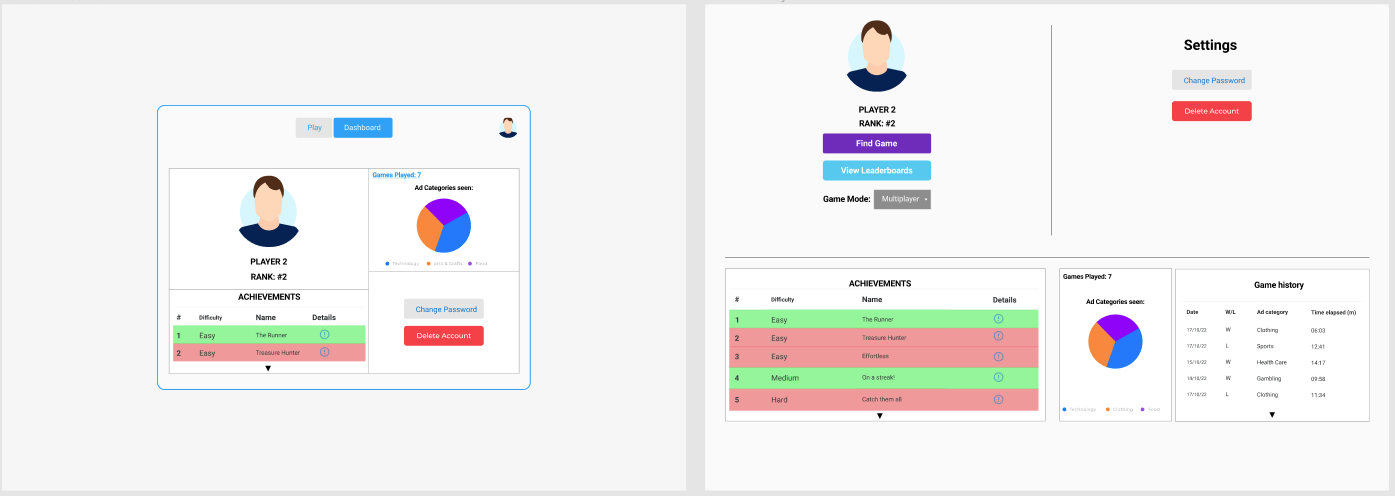
\includegraphics[width=1\linewidth]{images/Dashboard.png}    

    \caption{Two candidate designs for the dashboard page of the web app as they were presented to participants of the survey. Participants stated whether they preferred the left (Design 1) or right design (Design 2). }

    \label{fig:wireframe} 
\end{figure}

\begin{figure}
    \centering
    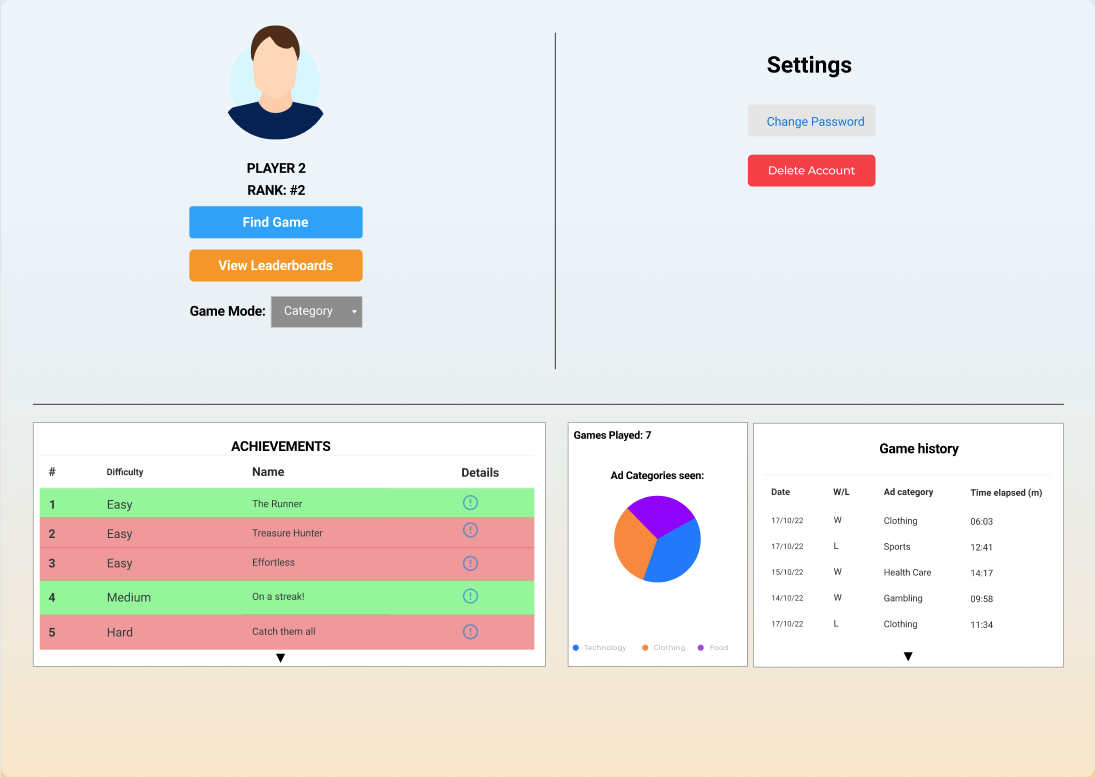
\includegraphics[width=1\linewidth]{images/DashboardFinal.png}    

    \caption{The prototype wireframe for the Dashboard after evaluation of the survey responses. }

    \label{fig:finaldesign} 
\end{figure}

\subsection{Web App Components}
The interface of the web app can be split into different components. We briefly mention these components along with any functionality they provide to the user.

\textbf{Authentication:} These are the register and login pages which will be the first thing new users will see when they visit the web app. New users can create accounts and existing users can use their credentials to log in, in which case, users are redirected to the dashboard.

\textbf{Dashboard:} The dashboard will be the main screen of the web app where most user interaction happens. In the dashboard, the user can search for games, view the leaderboard, game metrics, achievements and game history, change their profile picture or their password and find information on how to play.

\textbf{About:} The about page is the only page the user can navigate to other than the dashboard. It contains information about the concepts used in the game, as well as information about the game. The about page is meant to assist in improving the user's understanding of targeted advertising systems and the various issues involved with it. 

\textbf{Lobby:} When a user searches for and finds a game, they are redirected to the lobby. This lobby will allow players to chat with each other before the game or during the game. Players can see what the required winning condition is and indicate that they are ready for the game to start. When all players are ready, any one of them can start the game. During the game, players remain in the lobby, where they can continue chatting or choose to leave.

\textbf{Summary:} When a winner is found, players automatically get redirected to a summary page where they can see who won and their own or other players gameplay metrics. For example, in the case of the Race mode, users can see the pages other players have visited along with the number of unique trackers found in each page and their names. Players can continue chatting in the summary until they either choose to leave the summary page or play again. 

\section{Technologies used}
There were many technologies that we could have used for the development of the various components of the system. There were no limitations from the project specification, but since we are interested in tracking and 
advertising in web browsers, it was clear that we needed a JavaScript framework for the web application. Furthermore, to keep the language unified and consistent across our system components, we will also use a JavaScript framework for our
back-end, which will make it trivial to share resources between the server, client and extension using JSON data. 

\subsection{The Server}
The server needs to be able to handle authentication of users, communication between users and handle HTTP requests along with any database operations. Furthermore, since the game supports multiple players, we need
our server to be able to handle requests asynchronously so that it is non-blocking. The best choice for these requirements is implementing the server in Node.js along with Express since it provides most of the functionality we need out of the box, reducing the overhead
on additional libraries.  

\subsection{The Client}
The client needs to be able to handle all user interactions and display of information in the browser. There are a few different options we could have chosen for the client. The first option is vanilla JavaScript which is the most lightweight
with no overhead of additional libraries. However, with vanilla JavaScript it can be hard to implement more complex functionality. The second option is React, which is a component based web framework using a virtual DOM to render HTML 
content quicker. The third and final option is Angular, which supports two-way data binding, meaning that changes in the DOM will be reflected in the application code. However, Angular requires many libraries for efficient use, resulting in a lot
of overhead.

We have chosen to implement the client in React, as it is faster than Angular for smaller scale apps and supports real-time updates to the DOM using component lifecycles. Furthermore, using components will make development easier, as they
can be reused in different parts of the app.

\subsection{The Extension}
The extension needs to be able to handle all gameplay logic as well as displaying feedback to the users when they are in an active game. This means that it should be able to make updates to its interface that correspond to updates in the game state.
Therefore, we need our extension to have scripts running in the background that can handle the gameplay logic as well as scripts than can handle the updates to the interface. We have chosen to implement the extension in Google Chrome, as it is the
most widely used browser and the Google Chrome developer API provides many useful event driven methods that can help us detect trackers or identify adverts.

Google Chrome extensions are similar to web applications, in the sense that we can use web frameworks to implement them. However, for our extension we have chosen to go with vanilla JavaScript instead of using frameworks such as React or Angular.
This is because we are mostly interested in the scripts rather than the interface, and the Google Chrome developer API is powerful enough to help us implement the complex functionality required.

\subsection{Database}
For the relational database, we could have chosen any of the SQL databases as they all have the capabilities to handle any operation we might need for this project. However, for the selection of the database, we have decided to look ahead to the deployment of the 
app to avoid any potential incompatibilities between the service we will use to deploy the app and the database. 

A good service to deploy web apps that is free and supports automatic deployment is Heroku (\cite{heroku}). Heroku has add-ons that can be added to the deployed app which provide cloud databases that
our app can connect to. One of the most supported and commonly used add-ons is the Heroku Postgres which is what we will be using. Using PostgreSQL also makes it easy to store and query JSON data, which will be convenient when we want to store or retrieve entries for the game history.

%==================================================================================================================================
\chapter{Implementation}
\label{implementation}
What did you do to implement this idea, and what technical achievements did you make? 
React, Node.js-express, Chrome extension, postgresql database. 
Technical achievements:
- Three way communication between server, client and extension using http requests and websockets (can we break this down so that it is easy to explain and easy to grasp?)
- Ad tracker identification using Easy list
- Advert identification by looking at the dom (only a fraction of adverts, explain limits)
- Advert categorisation (web categorisation API). Explain approach and method
- Lobby system with real-time chat
- Achievement system
- Gameplay metrics, to analyse gameplay data in order to reach some form of conclusion (or identify any patterns in the players gameplay)

In this chapter we discuss the implementation details for the most important aspects of the different components of the system. We start by briefly explaining our software development process which was put in place to ensure that the project was organised and that most good software practises were followed.
TODO: \^ Refine statement above

\section{Software Development Process}

An important part of the software development process is being organised and following the best practises. We will briefly mention what our software development process was for this project before getting into the implementation details.

\subsection{Version Control and Agile Development}
For our version control we used GitHub (\cite{github}) as our remote repository. Most of the development and implementation of new features was done on the master branch. While we could have used a branching strategy to implement and test new features before merging them in the master branch, we did not feel like this was needed.

During the development of the product, we followed the Agile Scrum methodology (without the team roles) so that we could be flexible with the requirements as well as be organised with the tasks that we had to complete. Development happened in two-week sprints, where in each sprint we implemented one or more major features corresponding to the issues that were selected for that sprint. Issues were created to reflect the user stories during the requirement elicitation phase and further issues were created during development as necessary. 

GitHub provides a Kanban board which we used to organise issues into the backlog and the active sprint. For each sprint, issues were organised into four columns: To Do, In Progress, Done or Discarded. Each issue had additional labels denoting its priority, what the issue was about and what part of the system it affected. Since GitHub issues have no metadata for time tracking, we used a chrome browser extension called Clockify (\cite{clock}) to keep track of the time each issue took to complete. This allowed us to reflect on each sprint and ensure that time was spent on the more important issues. We also used Github's wiki to document any necessary aspect of the system as well as document our progress.

\subsection{Continuous Integration and Development}
An important aspect of Agile Development is CI/CD, which ensures that the implementation of new features does not break the functionality of the system. To deploy the app on Heroku, our repository had to have a specific structure, and therefore we created a deployment branch that has the appropriate code structure for deploying the app. GitHub actions allow us to define pipelines that execute a sequence of commands every time we push to the repository. We set up two different pipelines, one that run automated tests whenever we pushed to the master branch, and another pipeline that deployed the app on Heroku when we pushed to the deployment branch. This way, when the first pipeline failed, we knew that something had broken and we had to fix it before pushing to the deployment branch.

\section{WebSockets}
Before we begin explaining the implementation details for each component in the system, let us first discuss how we have implemented web sockets to handle the three-way communication between these components. We implement WebSockets using socket.io, which is a JavaScript library that provides an API to set up socket event emitters and event listeners. There are two different types of sockets, server-side sockets which will sit on the Node.js back-end and client sockets which will sit on the React front-end and the Chrome Extension for each of the users. 

Both types of sockets can emit events that the other type of socket can listen to, but client sockets can not listen to events from other client sockets. This means that for the client and the extension to communicate, they need to go through the server. This can be done by having event listeners on the server that listen to individual client socket requests and then emit an appropriate event to either a subset of the other clients or all of them, effectively allowing the client sockets to communicate indirectly.

From the user's perspective, they each have two sockets set up in their browser, one for the web app and one for the extension. The socket in the web app is mostly responsible for the chat, as well as reflecting updates to the game state in the web app. For example, when a winner is found, the extension socket notifies the server, which in turns notifies all connected clients and they are then redirected to the summary page. The socket in the extension is mostly responsible for sending game state updates to the server, which the server in turns sends to all connected extension sockets. It also has event listeners to identify when the game starts or when a user leaves the lobby so it can update its interface accordingly.

The server-side sockets are responsible for setting up the appropriate event listeners to handle the indirect communication between all client sockets. More details into what specific events are set up are given in the appropriate sections for each component.

\section{The Server}
The server uses Express along with Node.js to implement an http server and expose routes that the clients can consume through HTTP requests. To handle the requests, the server communicates with the database to retrieve any necessary information. Additionally, the server has utility classes to handle more complex functionality such as updating the user's achievements or dealing with the creation of lobbies. 

\subsection{Logging}
For each request made to our server, we keep a log that contains the request data as well as our server's response data. This makes it easy for us to identify and fix an potential errors in our server's controller logic. To do this, we define a middleware for each route that listens to an event indicating the completion of the request, and uses the data of the request and response to store entries in the database in the appropriate format.

Since we are interested in evaluating the system, we also store a log entry in our database for user interactions during gameplay. For example, when a user finds a unique tracker during gameplay, we store an entry to note the time and the website the tracker was found as well as the tracker's information. Since these interactions happen outside of the server and we need to store them in the database, we define a route that the react app can consume and send a request to the server to log a particular entry.

\subsection{The Lobby System}
To support multiple games being played at the same time, we had to implement a lobby system. The lobby system essentially puts users into different WebSocket rooms, which we call lobbies. When a user searches for a game, a lobby handler class either creates a new lobby if no available lobbies exists, or puts the user in an already existing lobby. Available lobbies are lobbies that are not yet full and are of the same game mode that the user selected. 

A lobby is its own class, and it is initialised by the lobby handler by passing in the game mode and an index which is used to differentiate between lobbies. The lobby also has attributes to store the users currently in the lobby, set the max number of players allowed in the lobby, and other useful game related attributes such as the winning condition for that lobby. The winning condition is selected randomly out of a subset of winning conditions when the lobby is first created. Appropriate methods are also defined to add or remove players from the lobby, and handle any other lobby functionality such as checking if the lobby is full or checking if all the players in the lobby are ready.

When the user is put in the lobby, their corresponding sockets are put into rooms. The browser socket is put into one room and it has event listeners and emitters to handle the chat functionality in the lobby, detect when a user leaves the lobby, detect when the game is finished and detect when all users are ready so it can enable the start game button which is disabled until all users are ready. The extension socket is put in a different room and has socket events to handle all the gameplay logic, update the game state for all players and detect when a game starts or finishes. The sockets stay in the rooms for the duration of the game as well as when the users are redirected to the summary page, since users can chat in the summary as well. When the users either leave the summary or leave the lobby during an active game, we remove their sockets from the rooms and remove the user from the lobby. When all users leave the lobby, the lobby handler destroys that lobby since it is no longer needed.

\subsection{Chat System}
Users that are inside a lobby have their browser socket inside the same room. When a user sends a message to the chat, their socket emits an event to the server with the information of the message. The server-side socket listens to this event, and then emits an event to all the remaining browser sockets in the room with the information of the message. The remaining browser sockets in the room listen to this event and append the new chat message to the chat container. Message information includes the user's username, the message that they typed and the date-time the message was sent. This allows the front-end to display who send the message, what the message is and at what time was the message sent.

The server can also chat with the players through its socket, and we do this to inform players that other players have joined or left the lobby.

\subsection{Updates to the state of the game}
When a game starts, an initial game state is created by the server that contains information about the players in that game, including their gameplay metrics such as the unique tracker count in the case of the Race mode or their page history. When the game starts, the server emits an event to all extension sockets to inform them that a game has started but also to send them the initial game state. During the game, when a player finds a new tracker, the extension increments their score in the game state by one and then emits and event to the server informing it that the game state of that player has changed. The server then emits an event to the remaining extension sockets with this new game state. The extension sockets then compare the new game state with their current game state and make the appropriate changes.

When a player wins the game, their extension socket notifies the server that a winner is found. The server then notifies all other players that the game is over and a winner was found and waits until all players have reported back their game state. When all players emit their game state to the server, the server puts everything together to create the final game state, which is used to create the summary page as well as the game history.

\subsection{Achievement System}
To handle updates to the player's achievements, we build an achievement handler which is a class that has methods to handle any achievement updates. The achievement handler executes its logic one step before players are put in the summary page. 

Each achievement has a condition which is an integer number that reflects the requirements of the achievement. An example achievement is "Play 5 games of the Race mode" and the corresponding condition would be 5. Furthermore, achievements have labels such as "race" to identify which metric to check against their condition, which allows us to dynamically check all achievements. The achievement handler takes in the final state of the game and for each player it retrieves their previous gameplay metrics and uses the gameplay metrics from the final game state to check if the player has passed the condition to complete an achievement. If a player had previously played 4 games of Race mode and has just finished another game of Race mode, for all achievement that have the "race" label, it would compare this new sum with the condition of that achievement and either mark the achievement as completed if the sum is more than or equal to the condition or mark it as In Progress if it is less. If no progress is made in a specific achievement then that achievement is marked as Not Started. This allows us to only check for achievements that have not yet been completed.

\subsection{User Gameplay Metrics}
Similar to the achievement handler, the user's gameplay metrics are updated one step before players are put in the summary page and it is a very simple process. A metrics handler class takes the final game state and for each user, it retrieves their previous gameplay metrics, adds to those metrics the metrics extracted from the final game state and updates the entries in the database. The metrics handler has appropriate methods to handle updates to the user's gameplay metrics for both game modes.

\subsection{REST API}

\subsubsection{Common Routes}
For the REST API, we define routes to retrieve, update and store information to the database tables. The routes are defined in separate controllers, for the different database tables. Each controller has methods that correspond to each route and return an HTTP response object, that contains a status of the request and the data that the client requested. For routes that require user authorisation, we use a middleware that checks if the request contains the appropriate and valid headers to confirm that the user is authorised, if they are not, they are redirected to the login page. 

\subsubsection{Gameplay Routes}
We also define routes that are not related to database tables, to handle complex game related functionality. When a user searches for a game, a request is made to the server with the user's information. The user then handles putting the player into the lobby and putting the player's sockets into rooms with the appropriate event listeners and event handlers. When all users are ready inside the lobby and start the game, a request is made to the server. The server then builds an initial game state with the appropriate data structures to store game related data and shares the initial game state with all players through their extension socket. For the remainder of the game, the server handles game state updates through the sockets until a winner is found. In the case of the Category game mode, the server has an additional route that handles the categorisation of adverts. These requests are made from the extension when an advert is identified during the game. The request contains the url of the advert's landing page. The server then queries the database to see if it had previously categorised that url, in which case, it retrieves its categories. If the url was not found in the database, the server makes a request to a web categorisation API that categorises the url and returns the categories or no category if it was unable to categorise that particular url. The server then stores a new entry for this url in the database and returns the categories.

When the game is over and a winner is found, the server then uses the final game state to build the game history and calls the appropriate methods to handle updates to the achievements and metrics of each player. Finally, the server emits an event to the browser sockets with the final game state and they are redirected to the summary page. The web app uses the final game state to display the appropriate information to the users.    

%\subsection{Error Handling}

\subsection{Database and ORM}
To implement our database models and handle database operations we use Sequelize which is on Object Relational Mapper (ORM) that functions as an interface between our server and our PostgreSQL database. Using an ORM instead of simply executing SQL statements to our database avoids the risk of SQL injections, but also makes it easier for us to define models by using the methods that Sequelize provides. We define a model for each database table with the appropriate fields as identified from the ER diagram we have created in the Design chapter. We further define the relationships between these models such that we can associate primary keys to foreign keys.

During development, we created a population script for our database that creates the database tables and also populates each database table with dummy data, or real data in the case of the achievement table which allows us to test that the database operations are functioning properly. 

\section{The Client}
Talk about the implementation of the client

\subsection{React Component Diagram}
In Figure \ref{fig:react}, we can see the React component diagram, showing the different components in the web app and the interaction between them. Each component is implemented as a JavaScript class that extends the React Component class and uses states and lifecycle methods to handle the logic and render the appropriate HTML content. 
\begin{figure}
    \centering
    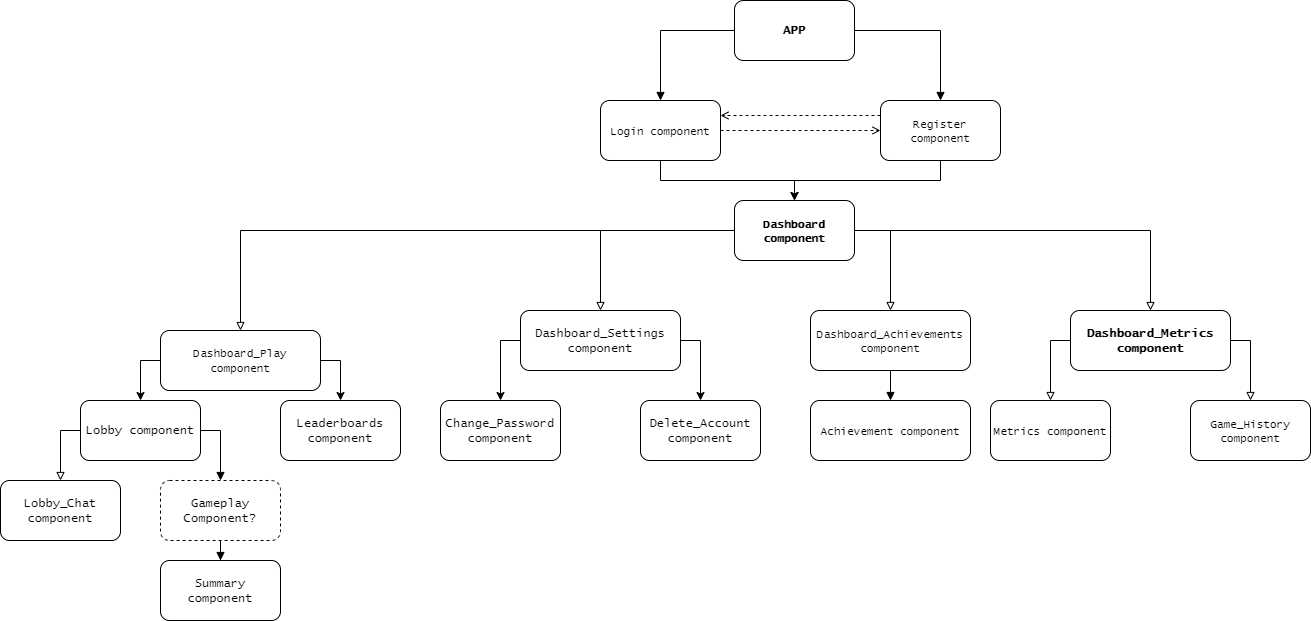
\includegraphics[width=1\linewidth]{images/react_comp_diagram.png}    

    \caption{React Component Diagram showing the hierarchy of the components in the web app, as well as the interactions between them. Arrows with a full black head means that the parent component navigates to the child component. Arrows with an open head means that the parent component is made up of the child components.}

    \label{fig:react} 
\end{figure}

\subsection{}

\section{The Chrome Extension}
Talk about the implementation of the extension

\section{Interface}
How did we implement the interface?

\section{Tracker identification}
Chrome extensions allows us to define scripts that run in the background, meaning that these scripts are active on all pages. To identify trackers we use a background script with two main functionalities, implemented by utilising the Google Chrome developer API. The first functionality is to ensure that the script only executes its logic when the player is in an active game. This means that the script should be aware when a game is active or not. To implement this we set up an event listener to listen for changes in the extension's local storage. We then check if there is any value changes to particular flags used to indicate that a game is active or not. Using these flags we can then decide when to execute the scripts logic. The second and most important functionality of this script is identifying and counting trackers while also emitting events to the server to update the game state for all other players. An event is also emitted to the server when the player wins. 

To identify trackers, we use a similar technique as that used by AdBlockers but instead of blocking the request, we simply count it. In particular, we set up an event listener that listens to the user's outgoing HTTP requests. For each of those request we extract the domain of the url the request is made at and compare it with a list that contains domains of known third-party trackers. If the domain we extracted is in that list, then that particular request was made to a third-party tracker's domain which effectively means they are tracking the user and therefore, we can add one to that player's tracker count. To make the gameplay more interesting and stop users from visiting the same pages, we only count unique third-party trackers, which are trackers that the user has not yet been tracked by during that particular game. If the domain we extracted is not in the list, then we simply move on to the next request until a winner is found.

\subsection{Page specific tracking}
When we extract the domain of the url the request is made at, we also extract the domain of the url the request is made from (the publisher's domain). We can then identify the page that a particular tracker was found which we use to build the summary as well as the player's game history. This is perhaps the most useful piece of information for the purpose of analysing the tracking done in different types of websites, as well as providing more transparency into the huge scale of tracking done to the players through the extension's interface.

\subsection{Optimizing the script}
To compare the url each request is made with the list of known tracker domains, we use the EasyList (cite). In its original form, it contains a list of regular expression rules that match the different urls that domain might have. This means that to identify a tracker, we had to execute each rule and see if we get a match. This was extremely slow, and it caused the browser to completely freeze up on websites that had a large number of outgoing HTTP requests.

It was clear that we had to further refine the list to optimize the speed at which the HTTP requests were processed. To do this, we had to utilise the domains of the urls since it is always the same regardless of the remaining url. We therefore created a script that iterates through the EasyList and for each regular expression rule we extract the domain, and create a mapping between the domain and the corresponding regular expression rule. We can then extract the domain from the url in the same way that we have extracted it from the regular expression rules to ensure consistency, and check for membership in this mapping in constant time, which solves the problem of being too slow.

\section{Advert identification and categorisation}
To identify adverts on different websites inside the browser, we needed a different type of script that has access to each website's HTML content and can execute its logic separately in each website. Fortunately, chrome extensions allows us to inject scripts in pages programmatically, and execute their logic once. We created a script that we only inject into pages when the user is in an active game of the Category mode. 

Advert elements are typically served to the user through HTTP response objects and they are nested inside multiple iframe elements, making it hard to detect. In addition to the advert elements, scripts are embedded inside the iframe to detect interaction with the advert. The structure of the iframe makes it hard to identify adverts, since there are no clear indications in the form of tags that would allows us to identify which element is the advert consistently. However, the advert element contains two children elements that we are interested in: A hyperlink with the url to the advert's landing page, and the advert's image element. Therefore, instead of looking through each element in the iframe, trying to detect adverts, we extract all the children hyperlink elements of the iframe and use a similar technique as that used by \cite{} in their AdReveal tool to identify advert urls. For each hyperlink, we extract the url and check whether that url contains the string 'adurl='. With this method, we can match adverts served by Google's DoubleClick, which is the most widely used ad exchange by publishers (\cite{dclick}}. However, we were unable to find any other consistent method to identify adverts from other ad exchanges which means our gameplay is limited only to adverts served by Google. During test runs of the gameplay, it became apparent that this was not destructive to the gameplay, as we rarely came across adverts that were not served by Google.

%==================================================================================================================================
\chapter{Evaluation} 
In this chapter we evaluate user's knowledge of targeted advertising systems before and after playing the game, as well as the usability of the system by conducting an experiment. However, we had trouble finding people to participate in this experiment and in total, 9 participants took part in the experiment. Due to the small number of participants and the fact that most participants were computer science students that were already exposed to these concepts through University classes, our evaluation is certainly not valid, as we require more participants with greater diversity to reach meaningful conclusions. 

\section{Experiment}
For the experiment, participants were asked to complete a survey. The survey included questions to evaluate the user's knowledge of targeted advertising systems, tracking and the privacy issues involved with these systems as well as questions to evaluate the system's usability in general. The survey first asked participants to rate their knowledge on a scale of 1 to 5 of various aspects of these systems as well as rate their technical proficiency. This allows us to explore whether people with higher technical proficiency are more knowledgable in these systems which is something we expect. The survey then included instructions on how to set up and play the game, and asked participants to play one game of the Race mode and read the information sections on the web app. After playing the game, participants were again asked to rate their knowledge on the same questions that they were asked before the gameplay. Finally, the survey included ten questions taken from the SUS questionnaire (\cite{sus}) to evaluate the system's usability.

A better experiment would have been to ask people to play multiple games, as they would get more familiar with the gameplay and perhaps understand these concepts better. However, due to the difficulty in finding participants and the amount of time it took to complete the experiment (20-30 minutes), we did not want participants to feel like they were asked to do too much or waste too much of their time, because they might simply choose not to take part in the experiment.

\subsection{User Knowledge Of Targeted Advertising System}
Figure x.x shows a table of the responses from all the participants that took part in the experiment. As we can observe from the table, almost all participants rated at least one aspect of these systems higher after playing the game. It is worth noting that for the few participants that rated their technical proficiency low, the increase in knowledge is more significant. An interesting result is that some participants rated their knowledge lower after playing the game. This might mean two things; either the participants made a mistake or they acknowledge that these systems are far more complex than they previously thought and identified that their knowledge of these systems is not as good as they previously thought.

These results do not tell us much and if we had more participants, with a better representation of the different groups of internet users, we could have made more accurate conclusions.

\subsection{Gameplay Analysis}
Here is the analysis of the gameplay. For each game, for each player, look at their gameplay and try to get some meaning out of it.
Questions include:
 - What did users first try? Did they quickly realise better strategies?
 - What is the most common pattern seen amongst users (if any?)
 - Length of games for players that played more than one game
 - 

\subsection{System Usability}
After playing the game, participants were asked to answer the 10 questions taken from the SUS questionnaire to evaluate the usability of the system. The responses to these questions can be transformed into a SUS score that indicates how good the usability of the system is. Table x.x shows the responses to each question for all the users along with their SUS score and the as well as what each question was. We calculate the average SUS score across all users and get a score of 80, which falls short of being excellent by 0.3, and it is classified as good according to SUS score labels. This means that users found our system quite enjoyable and easy to use and had not particular trouble using the different functionalities in the system.

\section{Unit Testing} 

%==================================================================================================================================
\chapter{Conclusion}    

\section{Summary}
Summarise the whole project for a lazy reader who didn't read the rest (e.g. a prize-awarding committee).

\section{Limitations}
Explain what were the limitations in this project, what could be done differently? 
Limitations:
 - tracker list not exhaustive
 - Identifying and categorising ads is difficult, limited to Google's doubleclick ads
 - The lack of participants and the problem with the existing participants

\section{Future Work}
For someone taking this project forward:
 - Explore more patterns for identifying adverts
 - Add more game modes and achievements
 - Maybe implement a new feature (look at Tally saves the internet)

\section{Final Reflections?}
Not sure if this paragraph will be included in the end, but here reflect on the project, did you learn anything new? Was it challenging? Refer from the project journal.

%==================================================================================================================================
%
% 
%==================================================================================================================================
%  APPENDICES  

\begin{appendices}

\chapter{Appendices}

\section{Ethics Checklist}


\includepdf[pages=-]{images/Ethics_Checklist.pdf}

\section{Design Evaluation Survey}

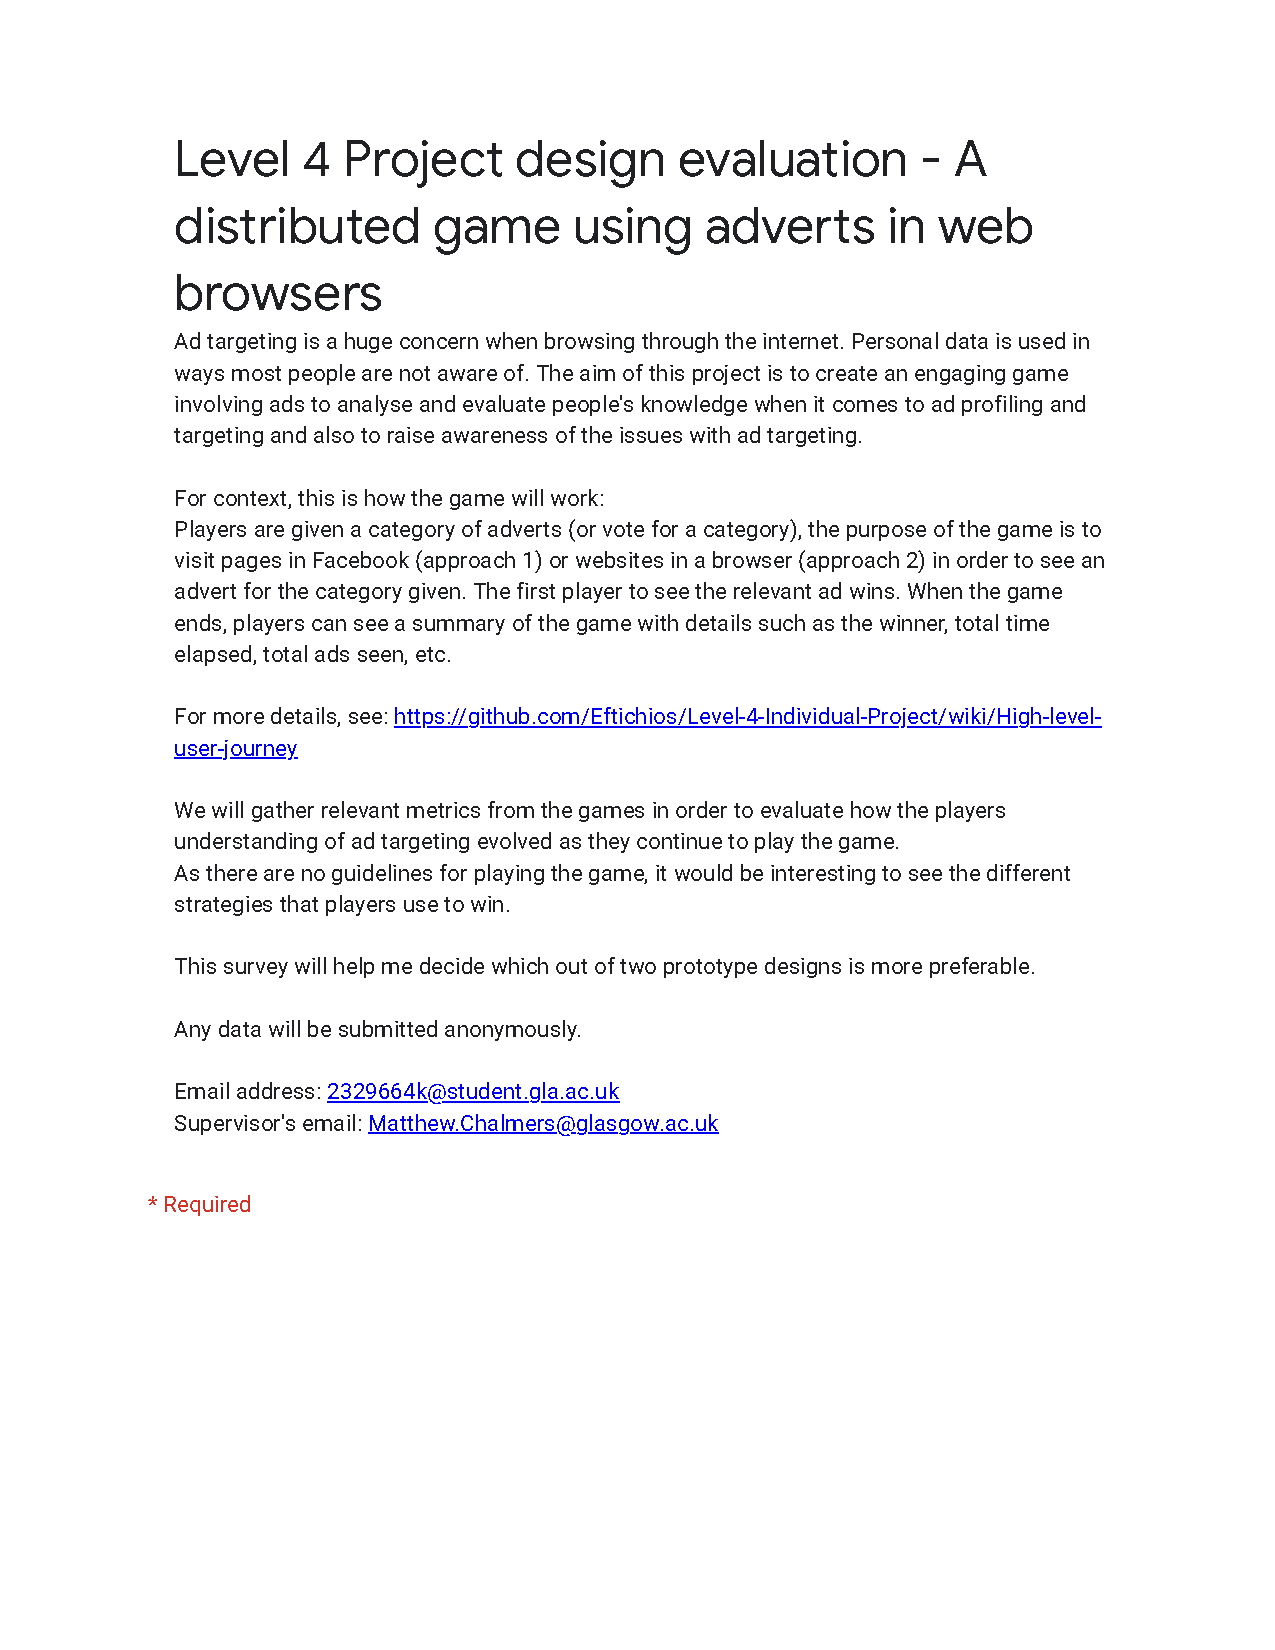
\includepdf[pages=-]{images/design_survey.pdf}

\section{Results For Design Evaluation}
TODO: Include tables and graphs of the responses gathered from this survey.

\section{Gameplay Evaluation Survey}

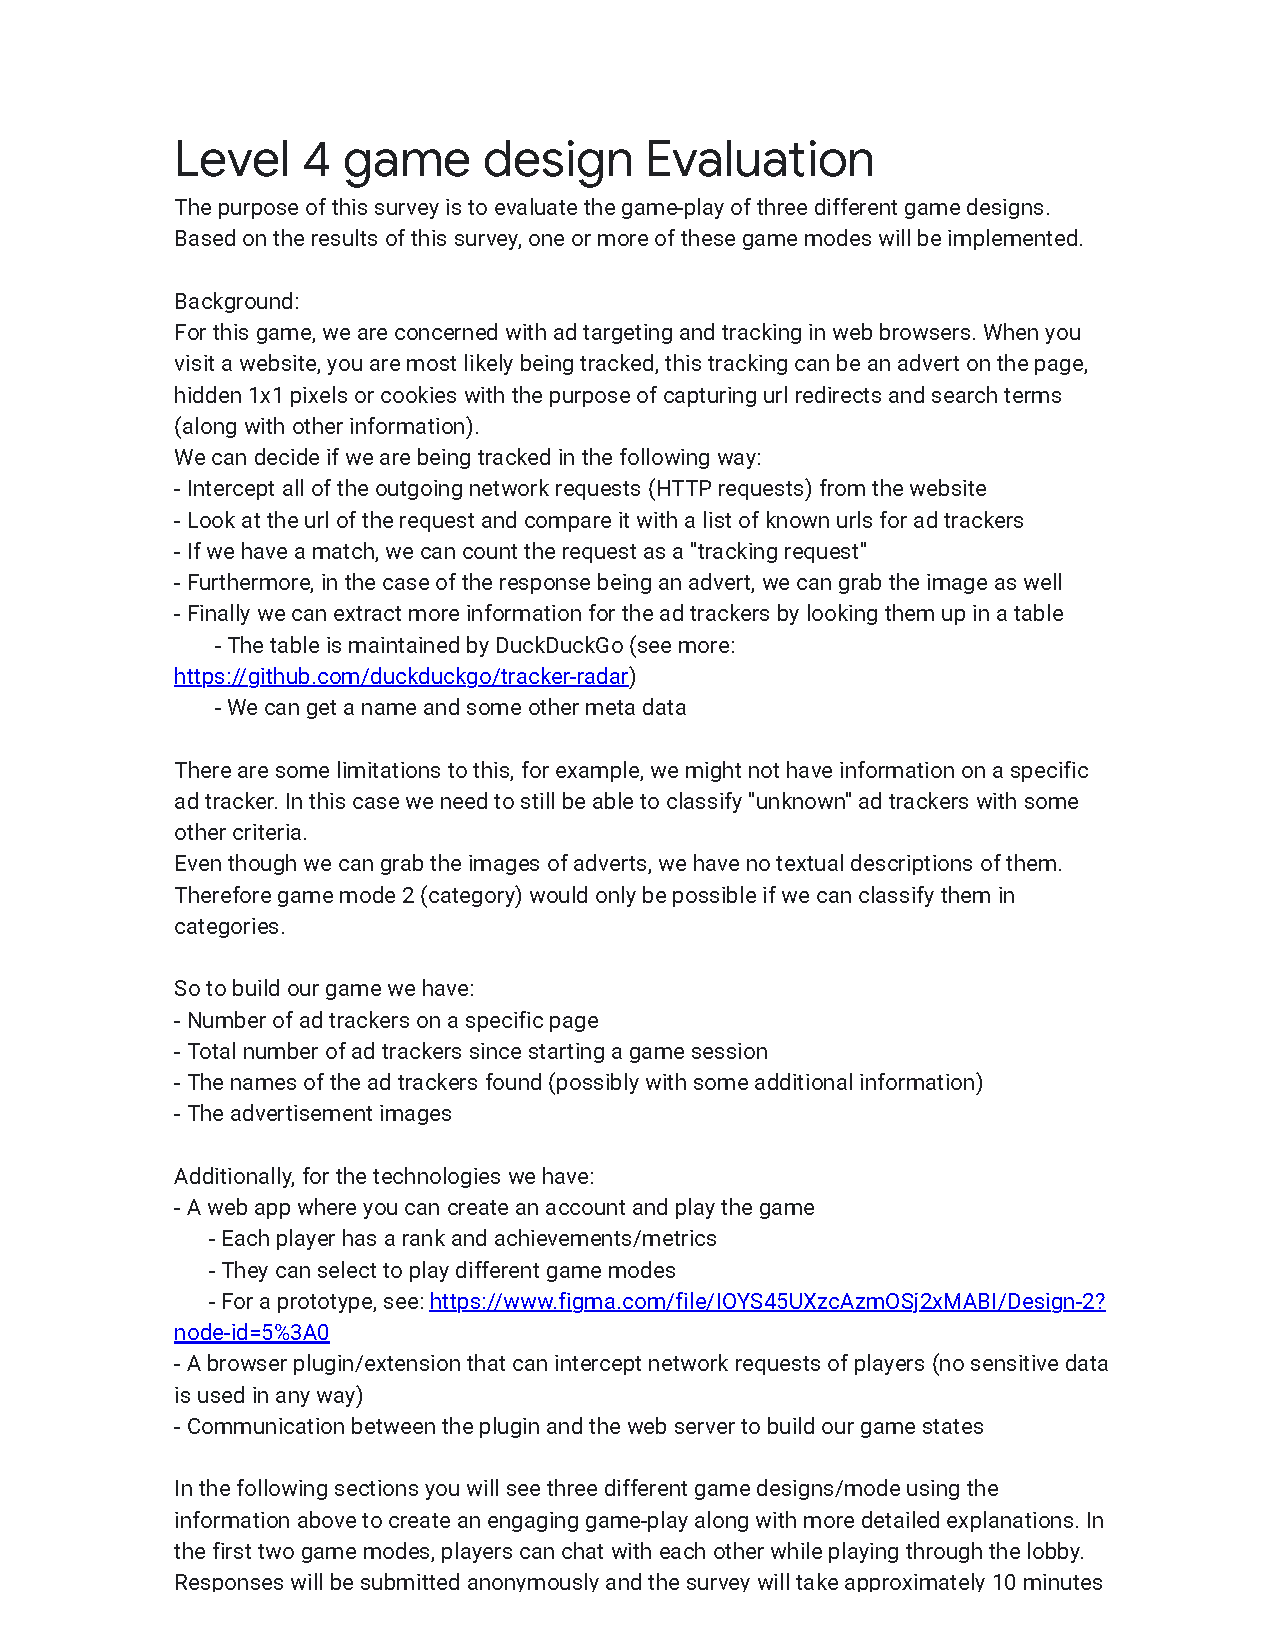
\includepdf[pages=-]{images/gameplay_survey.pdf}

\section{Results For Gameplay Evaluation}
TODO: Include tables and graphs of the responses gathered from this survey.

\section{User Evaluation Survey}

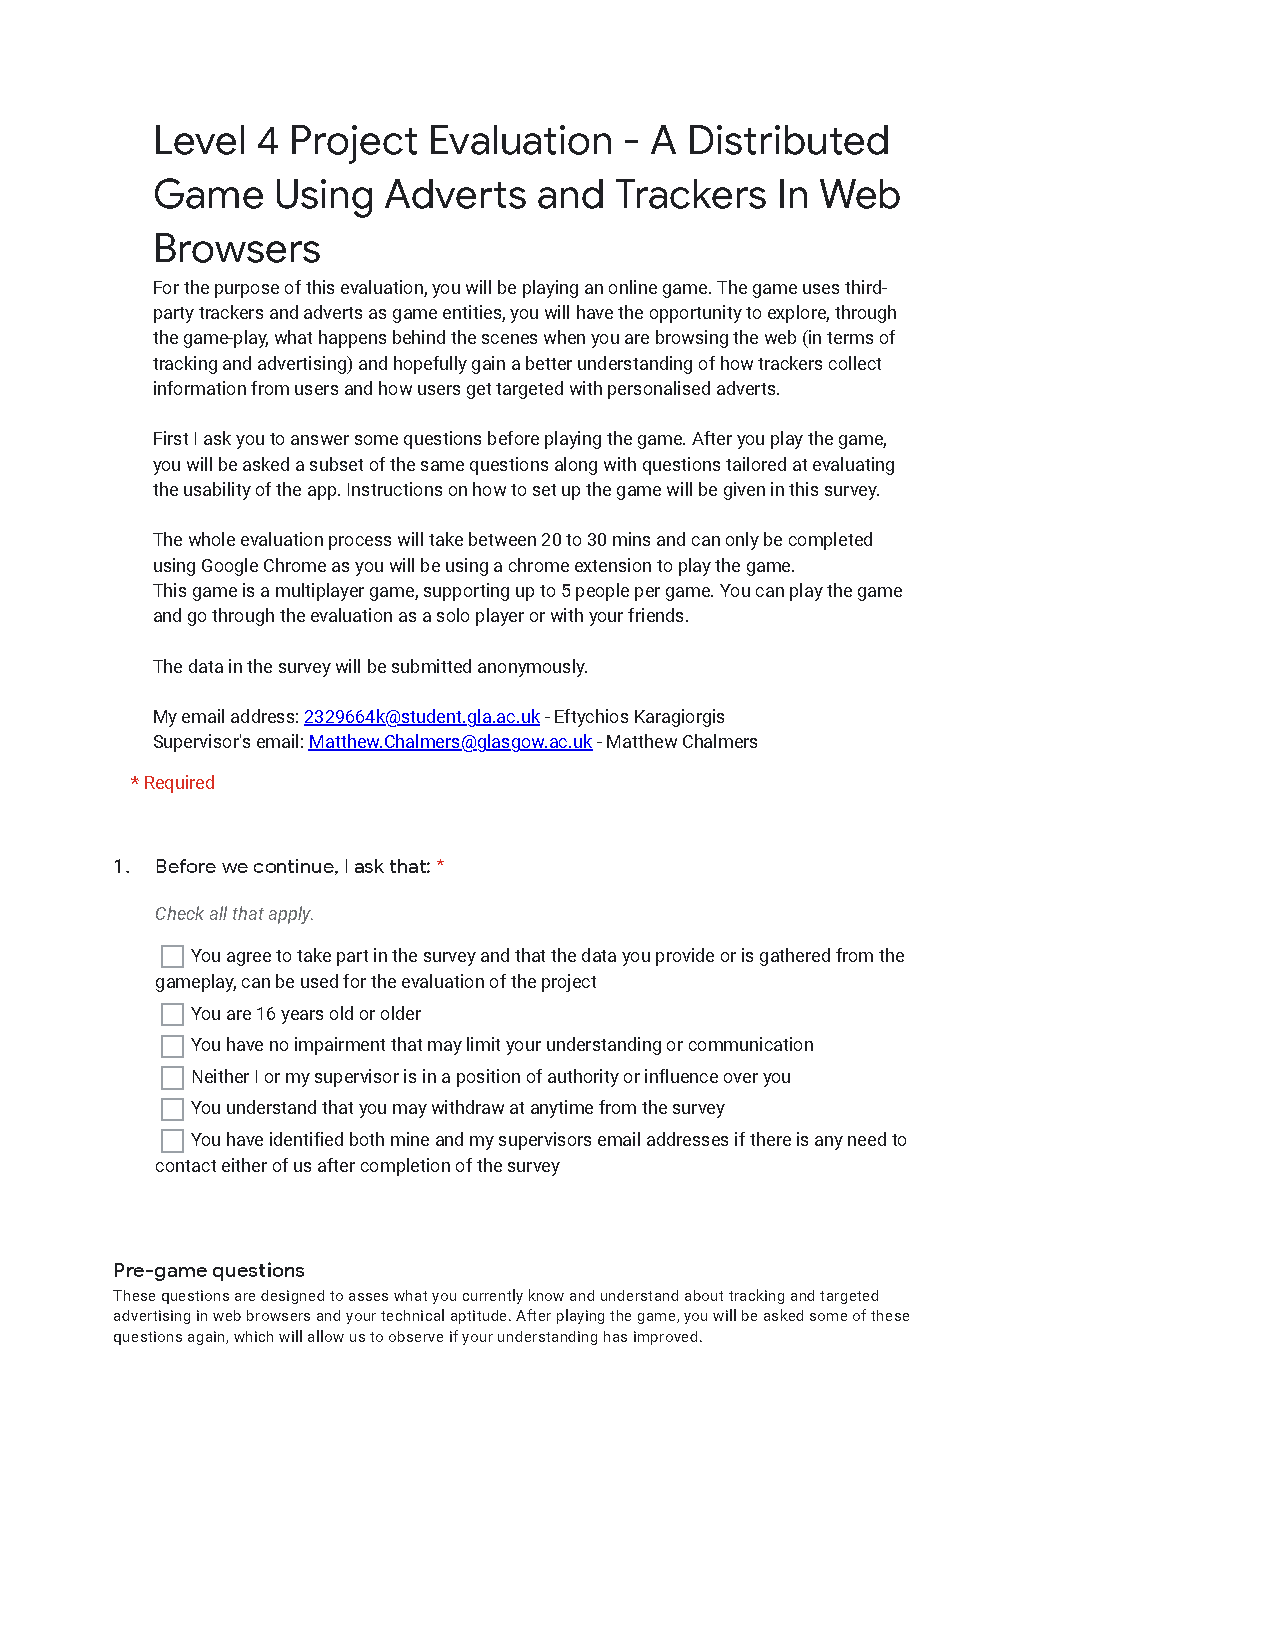
\includepdf[pages=-]{images/user_evaluation_survey.pdf}

\section{Results For User Evaluation Survey}
TODO: Include tables and graphs of the responses gathered from this survey.


\end{appendices}

%==================================================================================================================================
%   BIBLIOGRAPHY   

% The bibliography style is abbrvnat
% The bibliography always appears last, after the appendices.

\bibliographystyle{abbrvnat}

\bibliography{l4proj}

\end{document}
